\chapter{Réseaux de neurones pour le traitement de données biomédicales non-structurées}

\epigraph{\LARGE{``People should stop training radiologists now. It's just completely obvious that in five years deep learning is going to do betther than radiologists.''}}{\LARGE{-- Geoffrey Hinton, 2016}}


La vision de Geoffrey Hinton, lauréat du prix Turing 2018 pour ses travaux en \gls{ia} et en \gls{dnn}, était peut-être un petit peu optimiste. Presque huit ans après cette prédiction, les radiologues n'ont pas été remplacés par l'\gls{ia} et continuent d'être formés. Cependant il est important de remarqué que les méthodes \gls{ia} ont fait des progrès considérables et peuvent présenter des performances similaire aux radiologues, par exemple dans l'évaluation de radiographie de poumons (\cite{frauke_rudolf_ai_2023}). En juin 2023, il y a 238 produits médicaux basé sur IA pour la radiologies et autre méthodes d'imageries avec autorisation de mise sur le marche par la \gls{fda} (\cite{keith_j_dreyer_acr_2023}). Si l'\gls{ia} n'est pas encore prête à remplacer les radiologues et praticiens dans l'évaluation des données d'imagerie, elle est au moins maintenant capable de les assister afin de permettre un gain de temps et de précisions dans l'évaluation des données.


Au cours de la dernière décénie, le domaine de l'\gls{ia} a été révolutionné par l'apparaition des réseaux de neurones profonds (\textit{Deep Neural Networks}, DNN) grace notamment aux travaux des Yann Lecun, Geoffrey Hinton et Yoshua Bengio. Cette nouvelle technologie d'\gls{ia} fait une promesse intéressant dans le cadre des données biomédicales: être capable de traiter automatiquement des données non-structurée, c’est-à-dire sans devoir définir des descripteurs pertinents manuellement. Il est donc tout à fait pertinent d'explorer comment ces modèles peuvent être exploités pour le traitement des données biomédicales multimodales et hétérogènes. Dans ce chapitre nous allons d'abord présenter le fonctionnement des réseaux de neuronnes. Puis nous allons étudier deux architectures spécifiques de réseau de neuronnes qui ont permis la création de modèles d'analyse d'images (réseaux convolutifs)  et de texte libres (réseaux de types transformers).

\section{Présentation des réseaux de neuronnes profonds}

\subsection{Le concept de neurone et réseaux de neuronnes profonds}
Les réseaux de neurones sont un concept ancien qui ont été décrit pour la première fois en 1958 par Frank Rosenblatt (\cite{rosenblatt_perceptron_1958}) sous sa plus simple forme nommée le perceptron, un réseau composé d'un seul neurone formel. Les réseaux de neurones reposent sur le concept bio-inspiré des neurones. La figure \ref{fig:neurons} présente les similarité entre un neurones biologiques et un neurones formel en \gls{ia}. Le neuronne biologique via des processus biochimiques. Les signaux d'entrés des neuronnes précédants sont captés via les dendrites, intégré dans le corps cellulaire pour transmettre ou non un signal de sortie à travers l'axone vers d'autres neurones. Le neurone formel d'\gls{ia} est un modèle simplifié du neurone biologique qui mime leur fonctionnement. Ainsi le neurones formel intègre des entrées (x1, x2, x3 sur le schéma) comme les dendrites, calcul un signal à transmettre (via la somme pondérée des entrées et la fonction d'activation) comme le corps cellulaire et transmet ce signal aux neurones suivant (sortie) comme les axones.

Le perceptron, réseau de neuronne composée d'une seule couche de un ou plusieurs neuronnes entre l'entrée et la sortie, n'est efficace que pour traiter des problèmes à séparation linéaire. Pour traiter des problêmes de classification plus complexes, il est nécessaire de multiplier les couches de neuronnes entre l'entrée et la sortie du réseaux. Ces couches sont appelée couches "cachées", on a ici ce qu'on appelle un réseau de neuronnes profond. La limite entre réseaux de neuronnes classique (perceptron multi-couche) et réseaux de neuronnest profonds est floue. Certains auteur peut considérer un réseau de neuronnes comme profonds à partir de 3 couches cachées, d'autres 10 voir une centaine pour certains.

Similairement au cerveaux, ces neurones formels (artificiel) sont présent en grand nombre dans les réseaux de neurones profonds et sont interconnectés selon une organisation précise, cette organisation se nomme l'architecture du réseau.
\begin{figure}[!htbp]
 \centering
 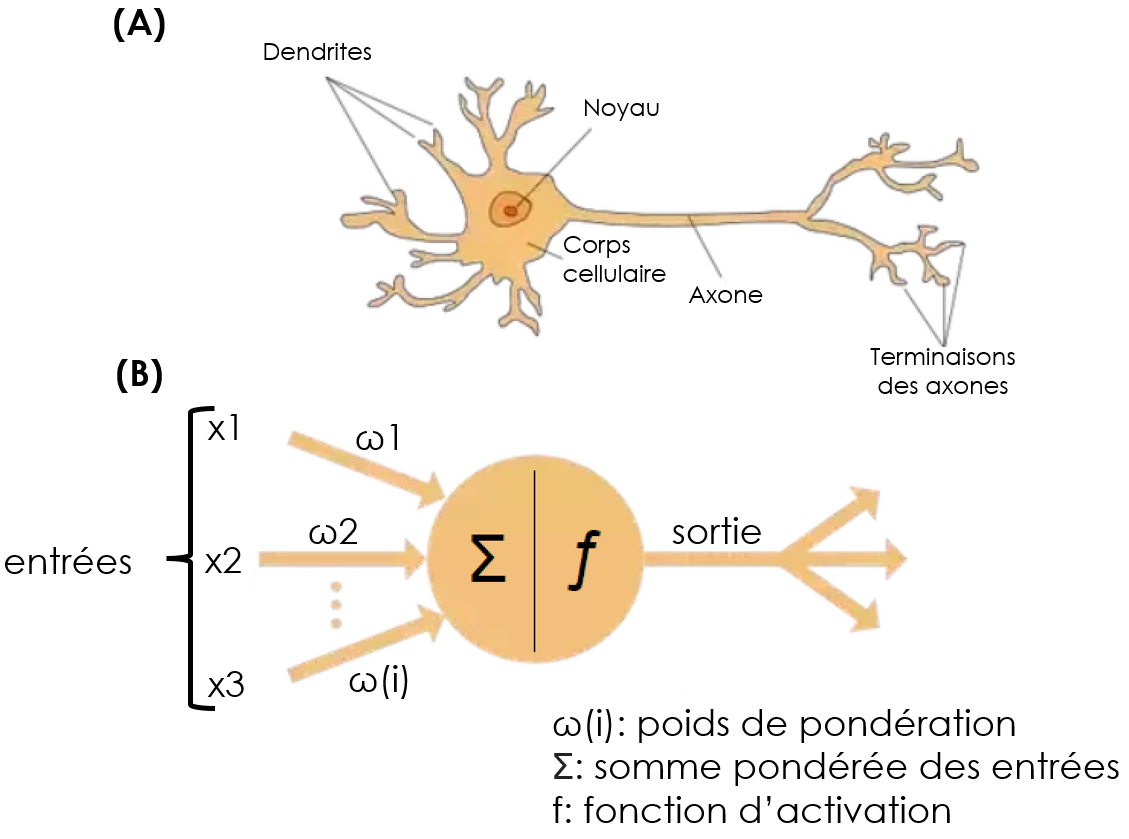
\includegraphics[width=0.7\textwidth]{figures/neuronne.png}
 \caption[Comparaison du neurone biologique et du neurone formel]{Comparaison du neurone biologique et neurone formel. (A) Représentation schématique du neurone biologique. (B) Représentation schématique du neurone formel utilisé en \gls{ia}}
 \label{fig:neurons}
\end{figure}
\subsection{Les réseaux de neurones: une diversité d'architectures}
La multiplication du nombre des neurones dans un réseau de neurones et de leur interconnection permet de constituer des architectures spécifique qui confère des compétences particulière au réseaux de neuronnes tels que l'intégration d'information locale (pour l'imagerie par exemple grace à la convolution, \cite{fukushima_neocognitron_1980}), l'intégration d'information globales (pour l'analyse de séquence par exemple grace aux \textit{transformers}, \cite{vaswani_attention_2017}), des mécanismes de "mémoires" (pour l'analyse de texte par exemple grace à la \textit{Long short-term memory}, LSTM, \cite{hochreiter_long_1997}) ou encore des capacités génératives (pour la génération d'images par exemples grace aux GAN et aux modèles de diffusion). La figure \ref{fig:dnn_archi} (\cite{leijnen_neural_2016}) présente graphiquement quelques architecture de réseaux de neurones communes. On y retrouve le perceptron (P), le perceptron multi-couches (DFF), le réseau LSTM, le \gls{dnn} convolutifs (DCN) et les réseau antagoniste génératif (GAN).

\begin{figure}[!htbp]
 \centering
 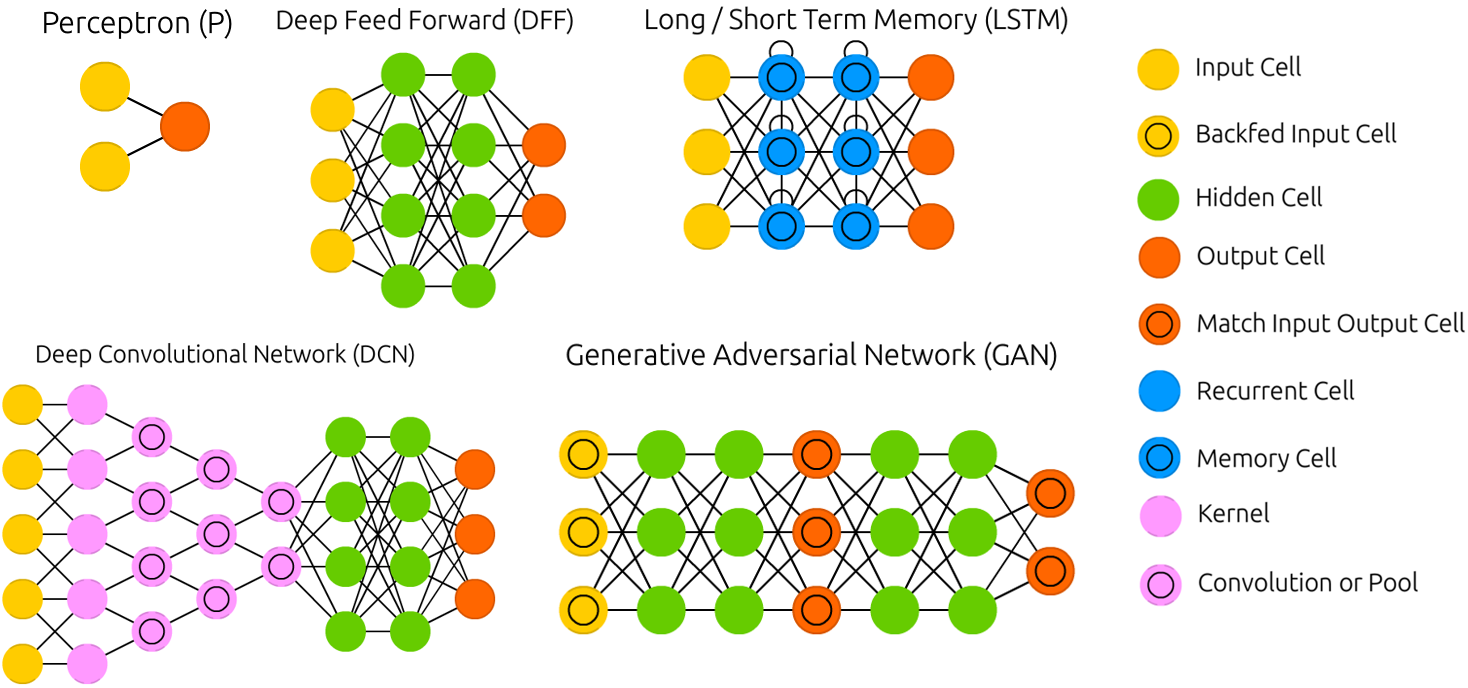
\includegraphics[width=0.9\textwidth]{figures/dnn_archi.png}
 \caption[Représentation de différentes architectures de \gls{dnn}]{Représentation de différentes architectures de \gls{dnn} (modifié de \cite{leijnen_neural_2016})}
 \label{fig:dnn_archi}
\end{figure}
multi layer perceptron d'abord le plus simple puis... convolution, transfermer, diffusion

\subsection{L'entrainnement d'un réseau de neuronnes}
L'entraînement d'un réseau de neurones consiste à trouvers pour chaque neuronne qui le compose, quel est la valeur de poids ($\omega$) pour chaque entrée optimale pour remplir la tâche qui lui est assignée. Pour cela un reseau de neuronnes a besoin de deux éléments: (i) une fonction de coût permettant d'évaluer son niveau d'erreur de classification et (ii) une méthode qui permet de modifier les poids des connections neuronales pour réduire cette erreure grace à la descente de gradient.

\subsubsection{Fonction de coût}
La fonction de coût permet de fournir une mesure quantitative des performances d'un réseau de neuronnes profonds. Elle mesure la divergence entre les prédiction réalisée par le modèle et les labels véritables des données. Cette fonction varie en fonction de la tâche à réaliser, pour une tâche de régression un choix courant est l'utilisation de l'erreur quadratique moyenne (\textit{mean square error}, MSE). Pour une classification il est commun d'utiliser l'entropie croisée binaire (\textit{binary cross entropy}). 
Dans tout les cas, plus cette valeur est élevée plus les prédictions du modèle divergent de la vérité de terrain, plus cette valeure est proche de 0 plus les prédictions du modèle sont exactes. Ainsi, l'objectif de l'entrainnement d'un réseau de neuronnes est de faire converger la valeur de la fonction de cout du jeu d'entrainnement et du jeu de validation vers 0. 

La figure\ref{fig:loss_func} présente un example théorique de valeur de fonction de coût au cours de l'entraînement d'un modèle \gls{dnn}. Dans cet exemple l'écart tout au long de l'apprentissage entre le jeu de validation et d'entrainnement est important à des fin de visualisaiton, en pratique les deux courbes doivent presque se superposer. On observe ici qu'au cours de l'entrainnement cette valeur converge vers 0. Cependant au bout d'un moment la valeur pour le jeu d'évaluation remonte tandis que celle du jeu d'entrainnement continue de baisser, il s'agit du phénomène de sur-apprentissage, le modèle cesse d'apprendreà généraliser et apprend simplement par coeur le jeu d'entrainnement. Ainsi il est necessaire d'arrêter l'apprentissage au moment ou la valeur du jeu de validation augmention, il s'agit de ce qu'on appelle l'arrêt prématuré pour éviter le sur-apprentissage.
\begin{figure}[!htbp]
 \centering
 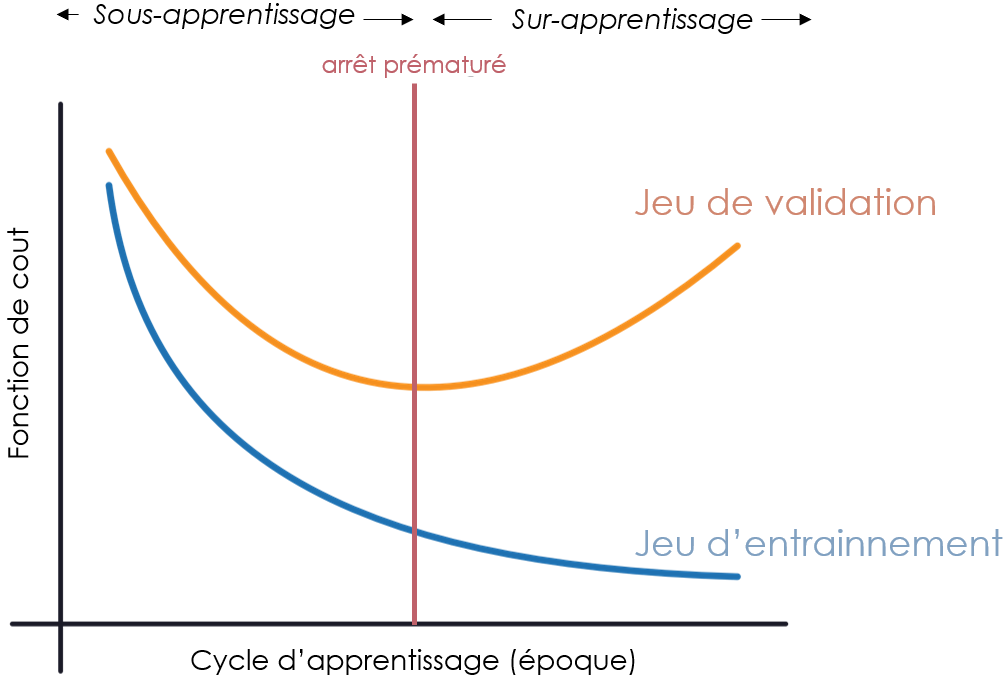
\includegraphics[width=0.7\textwidth]{figures/loss_function.png}
 \caption[Schéma d'un exemple de fonction de côut lors d'un entrainnement]{Schéma d'un exemple de fonction de côut lors de l'entrainnement d'un \gls{dnn}}
 \label{fig:loss_func}
\end{figure}
\subsubsection{Rétropropagation et descente de gradient}
La figure \ref{fig:retropop} (\cite{scalzitti_nouvelle_2021}) présente le mécanisme de rétropropagation. Lors d'une prédiction, les signaux sont propagés vers l'avant (nommé \textit{forward pass}) à partir de la couche d'entrée jusqu'à la couche de sortie, puis l'erreur est ensuite calculée grace à la fonction de coût. Lors de l'entrainnement, le chemin inverse est réalisé en propageant le gradient de l'erreur pour identifier les neuronnes responsable des erreurs (\textit{backward pass}) (\cite{lecun_deep_2015}). Ce processus de rétropapagation permet d'identifier quels sont les neuronnes responsable des erreurs dont les paramètres doivent être modifié pour réduire la fonction de coût.
\begin{figure}[!htbp]
 \centering
 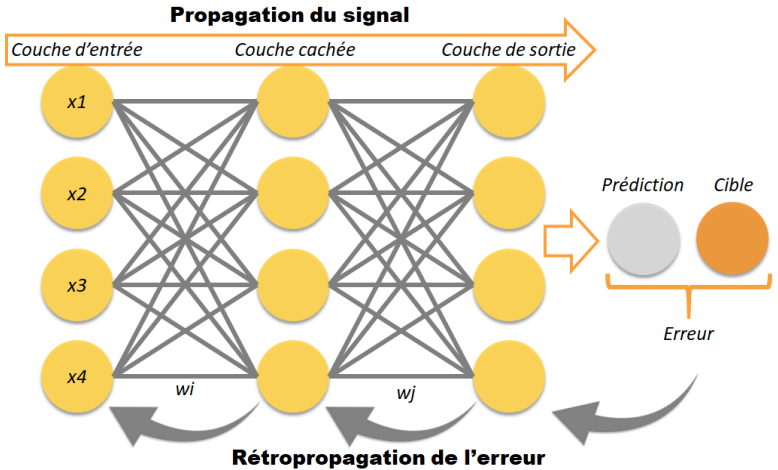
\includegraphics[width=0.7\textwidth]{figures/retro_propagation.png}
 \caption[Schéma de la rétro-propagation]{Schéma de la propagation du signal lors de la prédiction et de la rétro-propagation lors de l'entraînement (\cite{scalzitti_nouvelle_2021})}
 \label{fig:retropop}
\end{figure}
Après avoir identifier les neuronnes à modifier (et donc avoir calculé le gradient de chaque neuronne), leurs poids vont être ajusté grâce à la méthode de la descente de gradient. La figure \ref{fig:grad_descent} présente le fonctionnement de la descent de gradient. A chaque étape d'apprentissage les poids des neuronnes (ici un seul poids pour un neuronne sur la figure) sont mis à jour dans la direction négative du gradient, ce qui a pour effet de réduire la valeur de la fonction de coût. Cette modification des poids  proportionelle d'un paramètre nommé le pas d'apprentissage (\textit{learning rate}). Ces cycles d'apprentissage vont se répéter jusqu'à atteindre un minimum (global ou local) dans la fonction de coût, indiquant un poids optimal pour la fonction de côut (et donc la tache à réaliser).
\begin{figure}[!htbp]
 \centering
 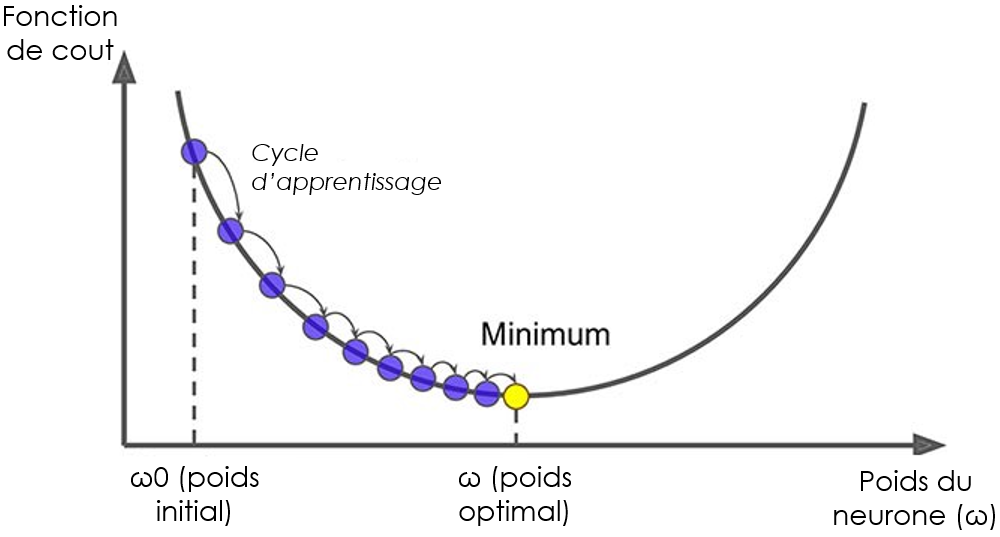
\includegraphics[width=0.7\textwidth]{figures/gradient_descent.png}
 \caption[Schéma de la descente de gradient pour un poids d'un neuronne]{Schéma de la descent de gradient pour un poids d'un neuronne}
 \label{fig:grad_descent}
\end{figure}

La rétroprogation et la descente de gradient permettent l'apprentissage de réseaux de neuronnes composés de centaines de miliers voir de milions et même de miliards de neuronnes. La taille des \gls{dnn} est très variable en fonction des architectures et de la tâche à effectuer. Ainsi les couts en calcul pour leur entrainement (le calcul des gradients et la mise à jours des poids) peut devenir très importante. Dans la prochaine sous-section nous allons plus réseaux et architectures de \gls{dnn} et les ressources informatiques associées nécessaire à leur utilsation.

\subsection{Nombre de paramètres et ressources informatiques}
Il existe un lien de proportionnalité entre la taille (en nombre de neurones) d'un \gls{dnn}, sa précision et les ressources de calculs nécessaires à son entraînement et inférence. En théorie plus un réseau est grand, plus sa capacité à capturer des relations complexes entre les données est importante et donc il peut atteindre une meilleure précision. Le tableau \ref{table:dnn-size} (\cite{chollet_keras_2023}) présente plusieurs architectures utilisée pour la classification d'image. On observe que pour une même architecture, augmenter le nombre de paramètres permet d'obtenir de meilleurs performances mais au cout d'un temps d'inférence plus long. Cependant lors d'une comparaison de deux architecture différentes, la relation performance - nombre de paramètre n'est pas forcément vérifiée. Les réseaux EfficientNet performent mieux que les réseaux ResNet avec un nombre de paramètre moindre, cependant une règle qui reste vérifiée dans toute les conditions: les réseaux qui performent le mieux ont un temps d'inférence plus long, quelque que soit leur architecture.

\begin{table}[!htbp]
\centering
\begin{tabular}{|l|c|c|c|} 
 \hline
 Architecture & Paramètres (Milions) & Précision (ImageNet, \%)  & Temps d'inférence (ms) \\
 \hline
MobileNetV2 & 3,5 & 71,3 & 3,8 \\
\hline
ResNet50V2 & 25,6 & 74,9 & 4,6 \\ 
ResNet101V2 & 44,7 & 77,2 & 5,4 \\ 
ResNet152V2 & 60,4 & 78,0 & 6,6 \\
\hline
EfficientNetB1 & 7,9 & 79,1 & 5,6 \\
EfficientNetB2 & 9,2 & 80,1& 6,5 \\
EfficientNetB3 & 12,3 & 81,6 & 8,8 \\
 \hline
\end{tabular}
\caption{Tableau de comparaison d'architecture de \gls{dnn} et performances (\cite{chollet_keras_2023})}
\label{table:dnn-size}
\end{table}

L'entrainnement et l'inférence des \gls{dnn} se réalise sur un matériel informatique spécialisé nommé \gls{gpu}. Au contraire des processeur (CPU) qui sont conçu pour des opératins séquentielles, les \gls{gpu} permettent de réaliser un grand nombre d'opération mathématiques en parallèle. Or, les opération principales nécessaires pour l'entraînement et l'inférence d'un \gls{dnn} sont des calculs matriciel et donc intrinsèquement parallélisables. La caractéristiques limitant des \gls{gpu} concerne leur mémoire disponibles (VRAM). En effet, plus le modèles de \gls{dnn} est grand, plus il possède de paramètre, plus il va est demandeur en mémoire, car il est necessaire de pouvoir stocker l'ensemble des poids à optimiser en mémoire. 

Ainsi, s'il est possible d'entrainer et de faire de l'inférence de modèle de taille raisonnable sur des \gls{gpu} accessibles au grand public, cette tâche devient complexe voir impossible pour des modèles de très grande taille sans engager des coûts de plusieurs centraines de miliers d'euro de matériel. A titre d'exemple, il est possible d'héberger et d'entrainnemer des modèles de quelques dizaines de milions de paramtères à quelques miliards paramtères (tel que Resnet50 (25M paramtères) et LLaMA-7B (7 miliards de paramtères) sur un seul \gls{gpu} grand public (16 à 24 Go de mémoire). 

Cependant plus récemment avec le développement des \gls{llms}, des modèles de plusieurs dizaine voir centaines de miliards de parmètres ont été entrainé et sont utilisé, comme par exemple GPT-3 d'OpenAI (175 milliard de paramtères \cite{brown_language_2020}) ou LLaMA de META (65 miliards de paramètres \cite{touvron_llama_2023}). Ce type de modèles demande l'utilisation de plusieurs \gls{gpu} haute de gamme (4 à 8) pour leur hébergement et inférence. A titre indicatif, un cluster composé de 4 \gls{gpu} H100 (40,000€ pièce), coûte 17.9\$/heure d'utilisation, soit environ 13 000\$ d'hébergement mensuel pour un modèle accessible en continu. Un travail d'optimisation pour réduire la taille des modèles tout en conservant leur performances est donc nécessaire pour permettre d'utiliser ce type d'architectures et d'outrepasser les challenges liés à leur hébergement.

\section{L'analyse d'imagerie par réseau neuronnal convolutifs}
L'architecture des réseaux de neuronnes convolitifs (CNN) permettent l'analyse et l'exploitation de données de types images brutes. Cette architecture est basée sur les travaux réalisée sur le cortext visual de chats et de primates dans lesquels il a été démontré que chaque neuronnes du cortext visuel captaient une information locale, dans un champs visuel réduit. Deplus chaque neuronne n'est en capacité de capter qu'une orientation de ligne (horizontale, verticales ou obliques) (\cite{hubel_receptive_1959, hubel_single_1959}). A partir de ces travaux, le concept de couches convolutive pour les réseaux de neurones a été formulé (\cite{fukushima_neocognitron_1980}) et a permis à la construction du premier \gls{dnn} convolutif pour reconnaitre des numéros sur des chèque de banque grace au réseau LeNet-5 (\cite{lecun_gradient-based_1998}). Vingt-cinq ans plus tard, en 2023, les\gls{cnn} sont encore utilisés pour l'analyse de données d'imagerie biomédicales (\cite{holscher_next-generation_2023, ker_automated_2019}).
 
\subsection{Fonctionnement des couches convolutives pour l'analyse d'images}
Pour simuler le comportement des neurones du cortex visuel, les neuronnes d'une couche convolutives ne sont connectés qu'à une zone restreinte d'une image, généralation sous forme d'un carré de pixels. La figure \ref{fig:conv_simple} présente schématiquement la liaison de trois neurones répartis sur deux couches convolutives par rapport à une image de base. On observe que ces neuronnes n'ont accès qu'à une portion de l'image, donc accès à une information locale. 
\begin{figure}[!htbp]
 \centering
 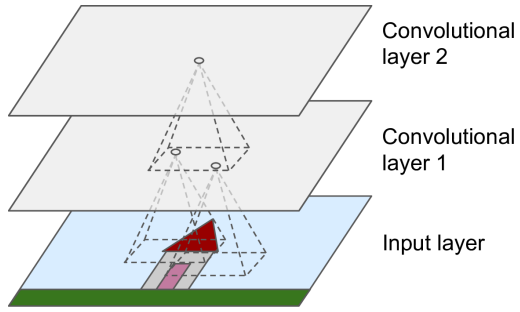
\includegraphics[width=0.7\textwidth]{figures/conv_simple.png}
 \caption[Schéma de la connection des neurones convultifs à une image]{Schéma de la connection des neurones convultifs à une image. Les neuronnes ne sont connectés qu'à une portion locale de l'image sous la forme d'un carré de pixels.}
 \label{fig:conv_simple}
\end{figure}
La convolution consiste à appliquer un filtre à une entrée pour produire une carte de caractéristiques (\textit{feature map}). Ainsi les neurones de la couche convolutive ont en entrée une portion de l'image et vont appliquer un filtre pour extraire une information de cette portion (une ligne horitontale, une texte, un contraste...). Le but de l'entraînement du \gls{cnn} est, pour chaque neuronne, de trouver quels sont les filtres optimaux à utiliser pour extraire l'information pertinente à la classification de l'image. Autrement dis chaque neuronne va apprendre à extraire une information pertinente de la zone à laquelle il a accès.

La figure \ref{fig:conv_simple} est simpliste, car elle représente les couches convolutives comme composée d'une seule couche de neuronnes et donc un seul filtre. En réalité, comme présenté en figure \ref{fig:conv_complex} chaque couche convolutives est composée de plusieurs filtres (couches de neuronnes formant des carte de caractéristique). Chacune de ces \textit{features map} est reliée aux précédentes afin d'extraire des caractéristiques très diverses (des formes horizontales, verticales, de la texture, du contraste...).
\begin{figure}[!htbp]
 \centering
 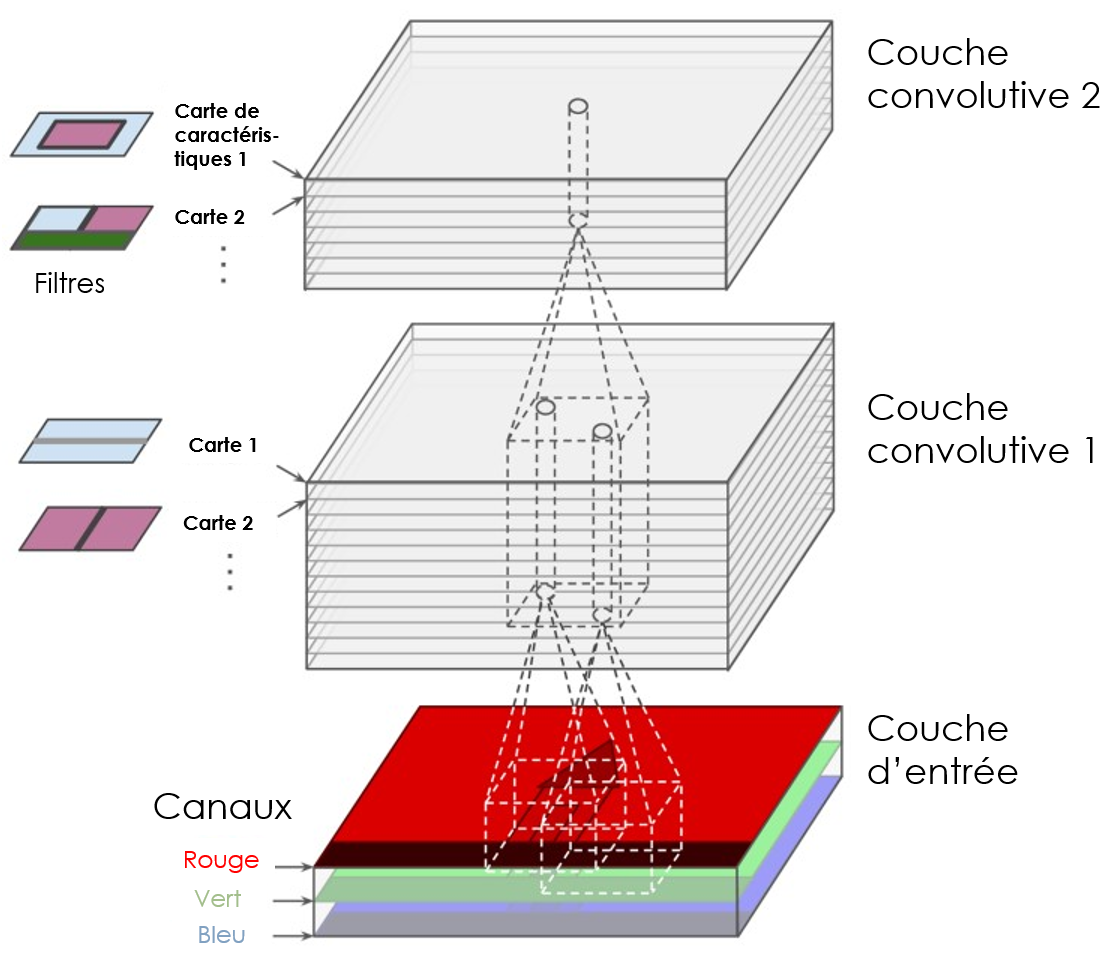
\includegraphics[width=0.7\textwidth]{figures/conv_complex.png}
 \caption[Schéma des couches convolutives]{Schéma des couches convolutives complexes.}
 \label{fig:conv_complex}
\end{figure}
Enfin pour simplifier les couts de calcul et réduire la mémoire nécessaire, après un bloc de covolution une étape de \textit{max-pooling }(en français: sous-échantillonnage maximal) est réalisée. Cette technique permet de réduire la dimensionalité des carte de caractéristique en préservant les informations essentielles. La figure \ref{fig:max-pool} présente le fonctionnement de cette méthode. La carte de caractéristique est divisée en carré non-chevauchant et la valeur maximal de chaque carrée est sélectionnée. Par exemple si on a une carte de caractéristique de taille 4x4 et qu'on réalise un \textit{max pooling} de taille 2, on obtient une carte de caractéristique de taille 2x2, c'est à dire quatre fois plus petite.
\begin{figure}[!htbp]
 \centering
 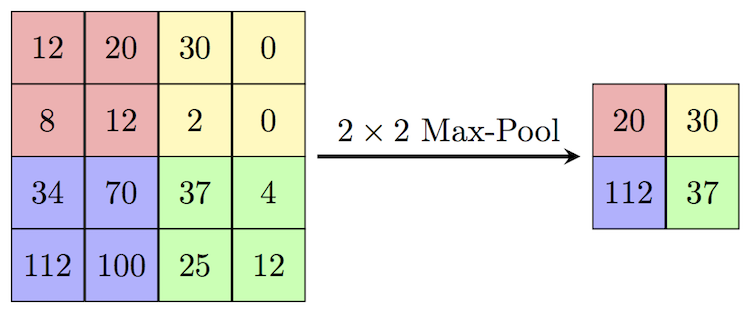
\includegraphics[width=0.5\textwidth]{figures/max-pool.png}
 \caption[Technique de max-pooling]{Schéma de la technique de max-pooling pour réduire la dimensionalité d'une matrice.}
 \label{fig:max-pool}
\end{figure}

Pour finir, la figure \ref{fig:cnn_archi} présente la structure typique d'un \gls{cnn}. Un \gls{cnn} consiste en l'enchainnement de couche de convulution et de \textit{max-pooling} avant le couches de classification (\textit{fully connected}). Le but de cette architecture est de réduire la dimensionalité de l'image tout en augmentant la profondeur (c'est à dire le nombre d'informations extraite par position). Ainsi par exemple pour une image de 512x512 (c'est à dire 262 144 pixels), si en sortie de couches convolutives on obtient une matrice de taille (4x4x128, soit 2048 points), cela signifie que nous avons extrait 128 caractéristiques pour chacune des 16 zones de l'image. Et ce sont ces 128 caractéristiques par zone qui vont être utilisée pour classer l'image.
\begin{figure}[!htbp]
 \centering
 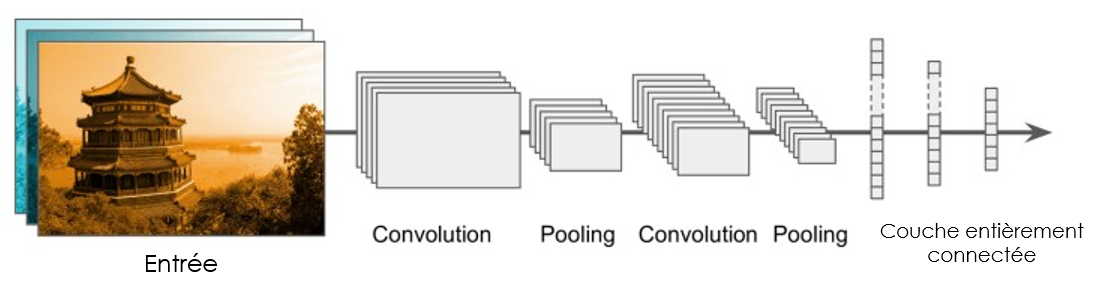
\includegraphics[width=0.7\textwidth]{figures/cnn_simple.png}
 \caption[Schéma de la structure d'un \gls{cnn} typique]{Schéma de la structure d'un \gls{cnn} typique}
 \label{fig:cnn_archi}
\end{figure}
\subsection{Modèle grand public pour l'histologie}
La couche de neurones convolutif représente la brique de base des \gls{cnn}. A partir de cet architecture de réseau il est possible de réaliser diverse tache en variant légèrement l'organisation des couches. Dans cette section nous présentons deux exemples d'utilisation des \gls{cnn} pour le traitement de données biomédicales.

\subsubsection{Segmentation d'images histologiques: détection de cellules avec Cellpose}
La segmentation d'une image consister à diviser l'images en groupes de pixels (segment) dans l'objectif d'obtenir les coordonnées d'éléments d'intérêts. Par exemple, dans le cadre d'une image de coupe histologique, il peut être intéressant de mesurer le nombre de cellules présente et leur taille. Pour automatiser ce processus, il est necessaire d'avoir recours à un réseau de neuronne capable de réaliser de la segmentation d'image.
Cellpose (\cite{stringer_cellpose_2021}), développé par Carsen Stringer en 2021, est un modèle de segmentation généraliste, conçu pour être capable de segmenter les cellules de n'importe quelle coupe histologique. La figure \ref{fig:cellpose_archi} présente l'architecture du modèle ainsi qu'un exemple d'image histologique et de résultat de segmentation. L'architecture de\gls{cnn} utilisée se nomme U-Net (\cite{ronneberger_u-net_2015}) structurée comme un U avec un chemin de contracteur (encodeur grâce à la convolution) et un chemin d'expansion (décodeur grace à la "\textit{upconvolution}"). Cette architecture permet à partir de l'image d'entrée, composée de cellules en microscopie à fluorescence, de générer un masque de segmentation, de la même taille que l'image d'entrée. Ce masque de segmentation est abstraction de l'image d'entrée où les pixels de chaque objet (cellules) sont marqués avec un identifiant unique. AInsi il est possible à partir de ce masque de compter ou de mesurer la taille des cellules.
\begin{figure}[!htbp]
 \centering
 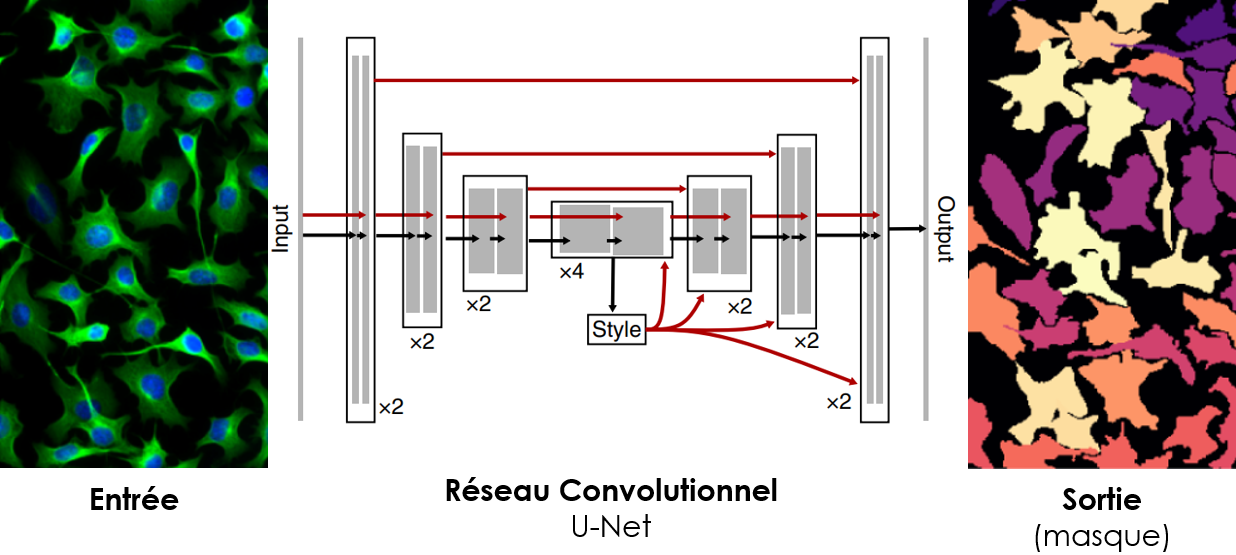
\includegraphics[width=0.8\textwidth]{figures/cellpose_archi.png}
 \caption[Architecture du réseau convolutionel de CellPose]{Architecture du réseau convolutionel de CellPose (modifié de \cite{stringer_cellpose_2021})}
 \label{fig:cellpose_archi}
\end{figure}
\subsubsection{Analyse de séquences: prédiction de sites d'épissage avec Spliceator}
\begin{figure}[!htbp]
 \centering
 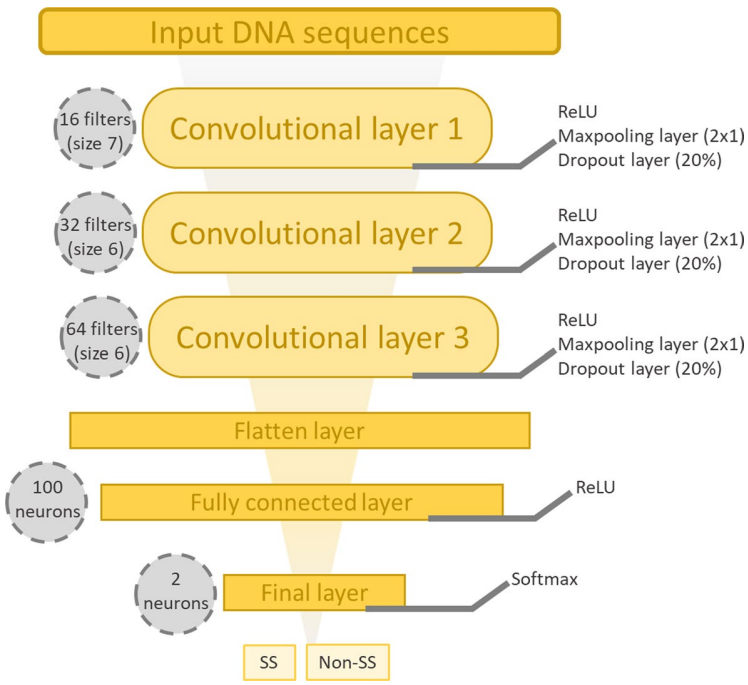
\includegraphics[width=0.66\textwidth]{figures/spliceator_nn.png}
 \caption[Architecture du réseau convolutionel de Spliceator]{Architecture du réseau convolutionel de Spliceator (\cite{scalzitti_spliceator_2021})}
 \label{fig:splice_archi}
\end{figure}

CNN cool mais information locales ça peut poser problême pour intéraction longue distance notamment, analyse de texte et de séquences. Introducing: les transformers. Dans la prochaine section nous allons voir une seconde architecture permettant de dépasser ces contraintes, capable d'intégrer des informations de contexte global.


\section{Architecture transformers et la révolution des modèles linguistiques de grande taille}
LLMs somme de deux choses: auto-supervisé + transformers 
 Plus récemment encore, grâce aux architectures à base de modules d’attention (\textit{Transformers}), des réseaux de neurones ont été entraînés pour comprendre du langage naturel (texte libre) et en extraire de l’information. 
https://huyenchip.com/2023/04/11/llm-engineering.html application des LLMs
\subsection{Modèle linguistiques de grande taille: la ruée vers l'or et modèles d'attentions}

L’année 2023 représente une année clé dans l’histoire du \gls{nlp} avec le développement et la mise à disposition de \gls{llms} généraux performants et accessibles tel que \textit{GPT-3.5-turbo (}souvent nommé à tort \textit{ChatGPT)} ou \textit{LLAMA}. 


\subsubsection{Exemple de transformers pour le triatement de séquences: AlphaFold}
\subsubsection{Exemple de transformers pour le triatement de séquences: Expression Enchancer}
\subsection{L'apprentissage auto-supervisé}
\subsection{Modèle génératifs, models embedding}
\subsection{Taille des modèles, hébergement, quantization}
\subsection{Exemple d'application en science}
DINO
SAM
Zero-shot, One-shot, Few-shot learning



Ces méthodes permettent d’explorer de façon rétrospective et multimodale, l’ensemble des données biomédicales acquises sur des patients sans avoir besoin de réaliser un travail manuel d’annotation trop important.